\usetikzlibrary{arrows.meta,calc,shapes.geometric}
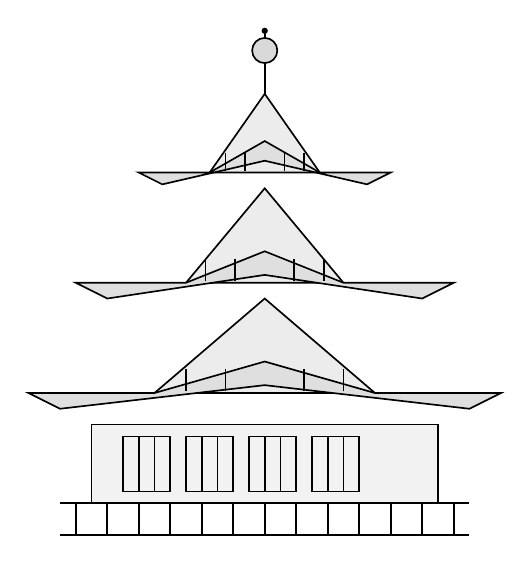
\begin{tikzpicture}[x=1cm,y=1cm,line width=.6pt,font=\normalsize]
\coordinate (F0) at (0.0,5.6);
\coordinate (F1) at (0.0,6.4);
\coordinate (R1L) at (-1.6,4.6);
\coordinate (R1R) at (1.6,4.6);
\coordinate (R2L) at (-2.4,3.2);
\coordinate (R2R) at (2.4,3.2);
\coordinate (R3L) at (-3.0,1.8);
\coordinate (R3R) at (3.0,1.8);
\coordinate (W0) at (-2.2,0.4);
\coordinate (W1) at (2.2,0.4);
\coordinate (W3) at (2.2,1.2);
% finial mast + ball (gray schematic of gilded top)
\draw (F0) -- (F1);
\filldraw[fill=gray!30] (0,6.15) circle (0.16);
\fill (0,6.4) circle (0.04);
% top tier: gable + flared eaves
\filldraw[fill=gray!15] (-0.7,4.6) -- (0,5.6) -- (0.7,4.6) -- cycle;
\filldraw[fill=gray!25] (-1.6,4.6) -- (-0.7,4.6) -- (0,5.0) -- (0.7,4.6) -- (1.6,4.6) -- (1.3,4.45) -- (0,4.75) -- (-1.3,4.45) -- cycle;
% mid tier
\filldraw[fill=gray!15] (-1.0,3.2) -- (0,4.4) -- (1.0,3.2) -- cycle;
\filldraw[fill=gray!25] (-2.4,3.2) -- (-1.0,3.2) -- (0,3.6) -- (1.0,3.2) -- (2.4,3.2) -- (2.0,3.0) -- (0,3.3) -- (-2.0,3.0) -- cycle;
% lower tier
\filldraw[fill=gray!15] (-1.4,1.8) -- (0,3.0) -- (1.4,1.8) -- cycle;
\filldraw[fill=gray!25] (-3.0,1.8) -- (-1.4,1.8) -- (0,2.2) -- (1.4,1.8) -- (3.0,1.8) -- (2.6,1.6) -- (0,1.9) -- (-2.6,1.6) -- cycle;
% ridge ornaments (schematic short ticks)
\foreach \x in {-0.5,-0.25,0.25,0.5} {
  \draw (\x,4.62) -- (\x,4.85);
  \draw (\x*1.5,3.22) -- (\x*1.5,3.5);
  \draw (\x*2,1.82) -- (\x*2,2.1);
}
% walls with lattice windows
\filldraw[fill=gray!10] (W0) -- (-2.2,1.4) -- (2.2,1.4) -- (2.2,0.4) -- cycle;
\foreach \x in {-1.8,-1.0,-0.2,0.6} {
  \draw (\x,0.55) rectangle (\x+0.6,1.25);
  \draw (\x+0.2,0.55) -- (\x+0.2,1.25);
  \draw (\x+0.4,0.55) -- (\x+0.4,1.25);
}
% balustrade base
\draw (-2.6,0.4) -- (2.6,0.4);
\draw (-2.6,0.0) -- (2.6,0.0);
\foreach \x in {-2.4,-2.0,-1.6,-1.2,-0.8,-0.4,0.0,0.4,0.8,1.2,1.6,2.0,2.4} {
  \draw (\x,0.0) -- (\x,0.4);
}
\end{tikzpicture}
